\documentclass[12pt]{article}
\usepackage[utf8]{inputenc}
\usepackage{graphicx} % Allows you to insert figures
\usepackage{amsmath} % Allows you to do equations
\usepackage{fancyhdr} % Formats the header
\usepackage{geometry} % Formats the paper size, orientation, and margins
\usepackage[style=authoryear-ibid,backend=biber]{biblatex} % Allows you to do citations - does Harvard style and compatible with Zotero
\addbibresource{Example.bib} % Tells LaTeX where the citations are coming from. This is imported from Zotero
\usepackage[english]{babel}
\usepackage{csquotes}
\usepackage{background}
\usepackage{minted}
\renewcommand*{\nameyeardelim}{\addcomma\space} % Adds comma in in-text citations
\linespread{1.5} % About 1.5 spacing in Word
\setlength{\parindent}{0pt} % No paragraph indents
\setlength{\parskip}{1em} % Paragraphs separated by one line
\renewcommand{\headrulewidth}{0pt} % Removes line in header
\geometry{a4paper, portrait, margin=1in}
\setlength{\headheight}{14.49998pt}
\backgroundsetup{scale=1,angle=0,opacity=0.175,contents={
\includegraphics[scale=0.25]{1200px-Vellore_Institute_of_Technology_seal_2017.png}}}


\begin{document}
\begin{titlepage}
\NoBgThispage
   \begin{center}
        \begin{figure}[h] % h - Place the float here, i.e., approximately at the same point it occurs in the source text (however, not exactly at the spot)
        \centering
        
\includegraphics[width=15cm]{1583124354phpJTtnK5.png}
        \end{figure}

        \Huge{Digital Assignment 1}

        \vspace{0.5cm}
        \LARGE{20BIT0406 - Sanchit Sandeep Khedkar}
       
        \vspace{2.5 cm}
        \Large{2022-02-28}
        
        \vspace{0.25 cm}
        \Large{ITE3001 - Data Communication and Computer Networks}
        \large{VL2021220500482 C1+TC1}
       

       \vfill
    \end{center}
\end{titlepage}
\newpage
\section*{The Data Link Layer}
The data link layer (DLL) is the second layer of the Open Systems Interconnection (OSI) Reference model. It is responsible for reliable passage of data frames from one node to another via the  physical  layer.  This  layer  is  largely  responsible  for sending raw data to the network layer. Data is communicated by  breaking  it  into  little  parts  known  as  packets, which  are then served to the network layer by the data link layer.Each frame
contains a frame header, a payload field for holding the packet, and a frame
trailer.Frame management forms the heart of what the
data link layer does.
\begin{figure}[h] % h - Place the float here, i.e., approximately at the same point it occurs in the source text (however, not exactly at the spot)
\centering
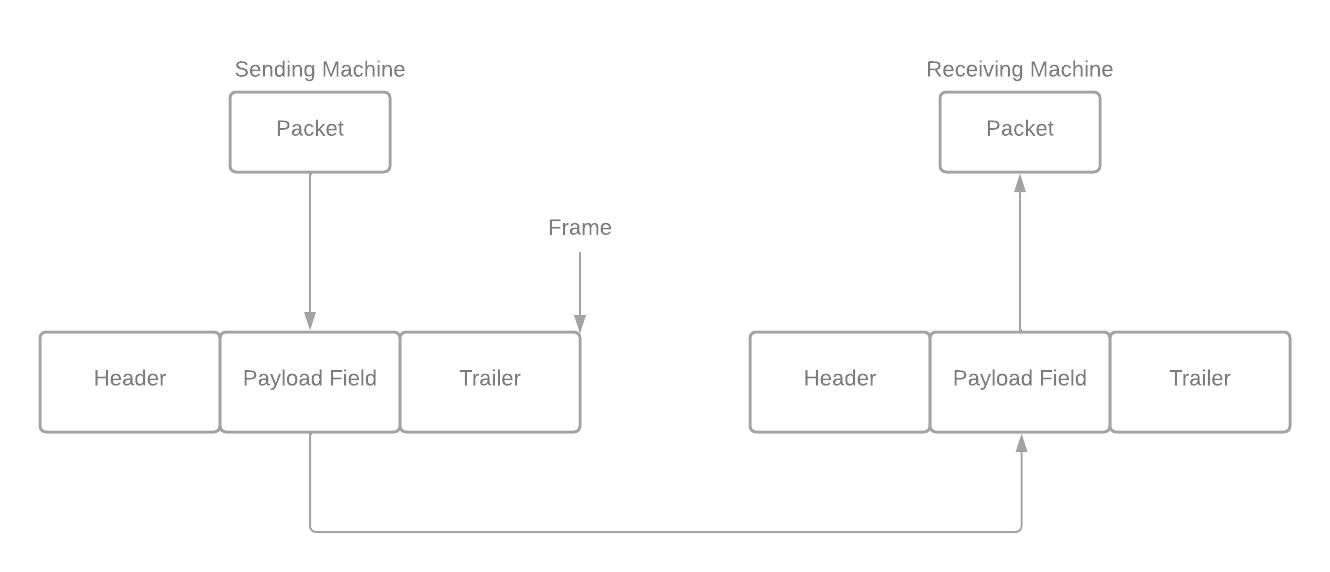
\includegraphics[width=\textwidth]{adslkfhkjalsdhf.png}
\caption{Relationship between packets and frames}
\end{figure}
The data link layer adds reliability to the physical layer by adding
mechanisms to detect and retransmit damaged or lost frames. It also uses a mechanism
to recognize duplicate frames. Error control is normally achieved through a
trailer added to the end of the frame.When two or more devices are connected to the same link, data link layer protocols are necessary to determine which device has control over the
link at any given time.
\\ \\
Even though the OSI Reference model was developed in the 1970s and 1980s there are still problems which persist and methods are being developed to counter such problems. The following text reviews such literature and provides an overview of them.
\setcounter{page}{2}
\pagestyle{fancy}
\fancyhf{}
\rhead{\thepage}
\newpage
The  Internet, a  rapidly expanding  communication infrastructure,  poses  significant  cybersecurity  challenges. A few techniques have been developed to provide security in the OSI model's application, presentation, and network layers. Implementing ECC on Data Link Layer of the OSI Reference Model; D. Ene, I. N. Davies, Godwin Fred Lenu, Ibiere Boma; SSRG International Journal of Computer Science and Engineering , 2021; recommends using public key Elliptic Curve Cryptography instead of using Media Access Control (MAC) to serve the Data Link Layer. It discusses the Address Resolution Protocol (ARP) and how attacks can happen through ARP, and also other attack routes. The paper expresses  the  synthesis  results  for  the  system implementation  and  shows  comparison  results  of  a secure data communication in the data link layer in the internet of things devices using Elliptic Curve Cryptography. The following tools were used to simulate the proposed system:\\
IAR Embedded Workbench: This is a toolchain that makes a complete IDE integrating all the tools in a single view, guaranteeing reliability, quality, and efficiency in the embedded application. It is a completely integrated development environment incorporating a compiler, assembler, a linker, and a debugger\\
Simulator: The simulator helped provide a realistic imitation of the operations and controls of the system. This tool simulated the programmable circuit board (PCB) and microcontrollers nicely but as a software.\\
Library Tools: All the required ISO/ANSI C and C++ source and libraries are included in the ECC libraries. This makes things very easy as there was not need recreating libraries.\\
ECC Parameters: 192 bits key length as recommended by the National Institute of Standards and Technology (NIST).\\
The following are the parameters of the encryption simulation.\\
a=-3\\
b=2455155546008943817740293915197451784769108058161191238065;\\
p=6277101735386680763835789423207666416083908700390324961279;\\
nB=28186466892849679686038856807396267537577176687436853369;\\
G= {60204628237568865675821348058752611191669876636884684818};\\
Pb= {2803000786541617331377384897435095499124748881890727495642}\\
The results were obtained simulating the overall system. The architecture was tested using files of the Wireshark logs as data link layer data sets. Signatures where generated and verified; also, files were encrypted and decrypted. The results were compared with results of the radio based wireless system. The results are displayed below
\begin{figure}[h] % h - Place the float here, i.e., approximately at the same point it occurs in the source text (however, not exactly at the spot)
\begin{subfigure}
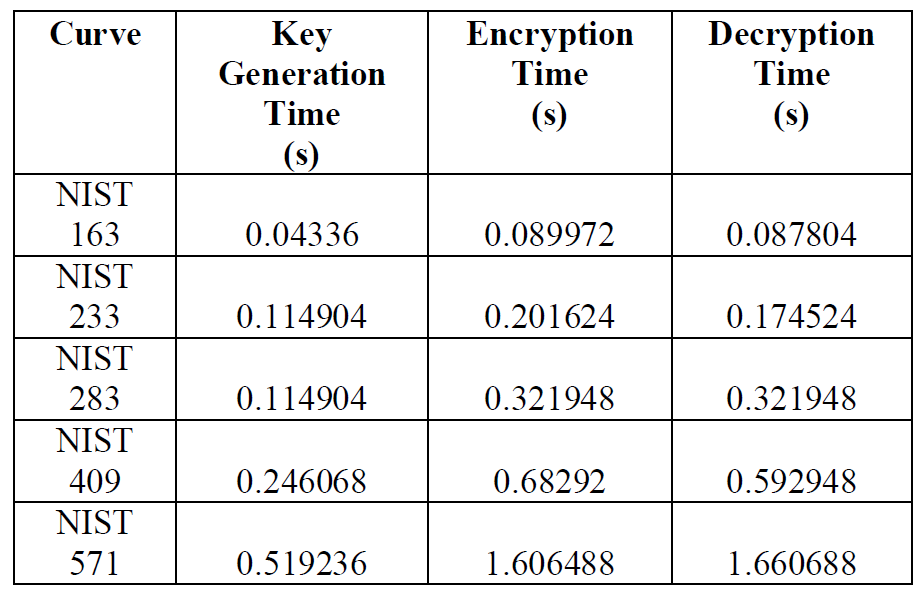
\includegraphics[scale=0.5]{Screenshot 2022-02-28 203107.png}
\end{subfigure}
\begin{subfigure} % h - Place the float here, i.e., approximately at the same point it occurs in the source text (however, not exactly at the spot)
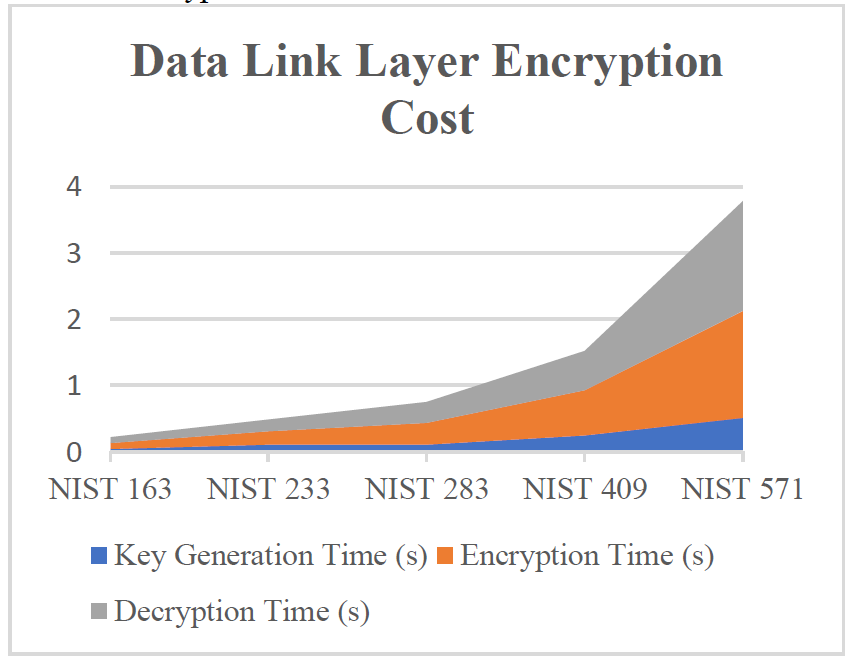
\includegraphics[scale=0.5]{Screenshot 2022-02-28 203116.png}
\end{subfigure}
\end{figure}
\\ \\
Implementation of Loop Prevention Protocols  at the Data Link Layer in LAN; Vladimir Dimitrov Dimitrov; 28-th National Conference with International Participation, 2020; discusses how In LANs, it is common for the network devices to be  interconnected  with  more  than  a  single  connection.  This way, even if a device or a connection fails, the network will continue  to  function  and  user’s  traffic  will  not  be  dropped, despite the minimal packet losses that would occur. However, another  problem  arises – loops. This paper examines the implementation and compression of protocols  such  as  MSTP  and ITU-T  G.8032  are  used  to  prevent  loops  in  such  networks. he MSTP protocol is implemented in a hypercube type topology to prevent looping at the data link layer. The  switches  are  interconnected  by  1  GE  (Gigabit Ethernet)  channel  bandwidth  optical  cables.  Some  of  the devices  are  interconnected  by  two  or  three  port aggregations - ag2 aggregation with two ports is used for connection  between  M2  and  M6,  ag3  aggregation  with three ports is used between M2 and M3, ag9 aggregation is used between M6 and M9 with 2 ports, between M1 and M12 aggregation ag12 with two ports is used. The  ITU-T  G.8032 protocol is implemented in a ring topology to prevent looping at the data link layer. The  switches  are  interconnected  by  1  GE  channel bandwidth  optical  cables.  Some  of  the  devices  are interconnected  by  two  or  five  port  aggregations  -  ag11 aggregation with two ports is used for connection between R1 and R2, ag1 aggregation with five ports is used between R1 and R9. In both protocols, tests were performed using network traffic in different VLANs and respectively different instances of the protocol. The time intervals for MSTP and ITU-T G.8032 respectively are displayed below
\begin{figure}[h]
\begin{subfigure}
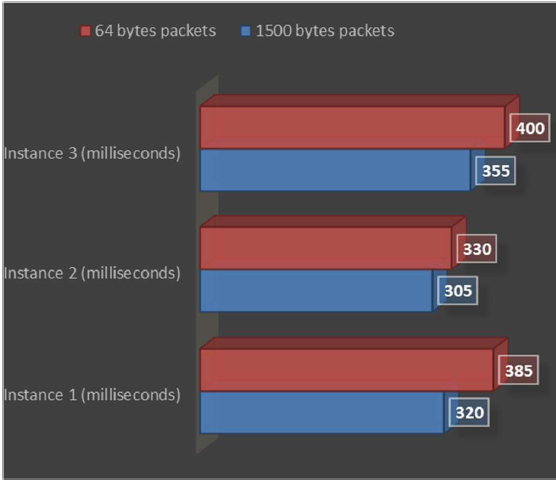
\includegraphics[scale=0.5]{Screenshot 2022-02-28 205131.png} 
\end{subfigure}
\begin{subfigure}
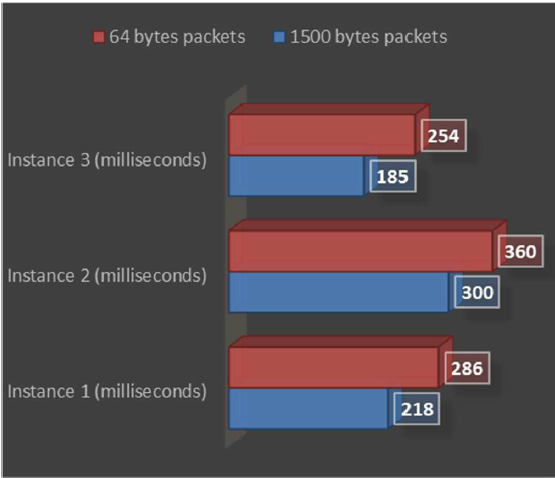
\includegraphics[scale=0.5]{Screenshot 2022-02-28 205204.png}
\end{subfigure}
\end{figure}
\\ \\
Development of Recommendations for the Implementation of Integrated Security in the Corporate Network at the OSI Data Link Layer; Kyryl Nikolchev, Kostiantyn Herasymenko, Olena Starkova, Mykola Yastrebov; 2020 IEEE International Conference on  Problems of Infocommunications. Science and Technology; argue that Layer 2 is considered to be the weakest link in OSI   model   because   LANs   traditionally   were   under   the   administrative  control  of  a  single  organization  where  all  persons  and  devices  were  trusted.  Today,  with  the  newest  attacks,  LANs  became  more  vulnerable  to  penetration.  OSI  Layer  2  solutions  are  not  effective  unless  the  management  protocols  are  secured and analyse  vulnerabilities  at  the    Data    Link    Layer    and    describes    ways    to    secure    management protocols. The literature discusses CAM table attacks, VLAN attacks, DHCP spoofing and DHCP starvation attacks, ARP attacks, and STP manipulation attacks. They then discuss CAM table attack mitigation which includes port security; VLAN attack mitigation by iterating the need to  disable  DTP  negotiation  (non-trunking)  on  non-trunk  ports  using  the  switchport  mode  access  command,  manually  enable  the  trunk  channel  on  the  connecting  port  using  the  switchport  mode  trunk  command,  disable  DTP  (automatic  trunking)  negotiation  on  trunk  ports  using  the  switchport   non-negotiate   command,   set   for   your   own   VLANs  different  from  VLAN  1,  set  for  unused  VLANs  using    the    switchport    command    trunk    native    vlan    vlan\_number  and  disable  unused  ports  and  place  them  in  an unused VLAN; DHCP attack mitigation by snooping  on  trusted   ports.   DHCP   tracking   creates   and   maintains   a   DHCP tracking binding database that the switch can use to filter  DHCP  messages  from  untrusted  sources.  The  DHCP  snooping  binding  table  includes  the  client's  MAC  address,  IP   address,   DHCP   lease   time,   binding   type,   VLAN   number,     and     interface     information     for     untrusted     switchports and interfaces; STP attack mitigation by  recommending  to  use  Cisco STP stability mechanisms to increase overall switch performance  and  reduce  the  time  lost  during  topology  changes.    It    is    recommended    to    use    STP    stability mechanisms:  PortFast,  BPDU  Guard,  Root  Guard,  Loop  Guard.
\\ \\
Research on a Certainty Data Link LayerProtocol for the Communication Networkin Nuclear Safety DCS; Le Li, Chun-Lei Zhang, Kang Cheng, Xing-Xing Sun, Wen-Yu Yang; Springer Nature Singapore Pte Ltd. 2020; argue that with the development of digital instrument and control (I&C) technology for nuclear power plants in recent decades, communication networks have become an important part of safety digital control systems (DCS). The certainty of the protocol is the main difference between nuclear safety communication and other industrial communication networks. A particular safety communication protocol which is designed and applied in data link layer(DLL) in communication network in safety DCS is proposed in this research. The literature discusses the certainty required by standards and regulations and talks about the various factors influencing the certainty of protocols. It then discusses the solution to certainty safety communication protocols by first discussing the topology and model of the communication network and then DLL functions in detail, including DLL function modules, service interfaces, communication scheduling mechanisms, frame structures and argues that the implementation of the function does not depend on the specific implementation strategy, but must be implemented in the communication protocol. The proposed safety communication protocol with the FirmSys, the first safety DCS produced by China with proprietary intellectual property, was simulated by a discrete event-based simulation model. In addition, the full-coverage verification of the protocolwas performed using a formal verification technique based on model checking, which could guarantee the high certainty of the safety protocol. Finally, a comprehensive and in-depth practical testing had been taken for more than three years, using the communication network devices of the FirmSys to build a fully configured network prototype. all nodes are sequentially connected, which composes a safety ring network with a configurable number of nodes. Achieving a communication rate of 1 Gbps, the maximum update time of node data is less than 5.5 ms, under the configuration of 48 nodes. The transmission time with a particular application where ten communication pockets would be required to transmit is also tested, and the result is shown. As a result, the maximum update time of node data is less than 7 ms with the testing prototype, which indicates that the proposed protocol could ensure the certainty of the safety communications.
\begin{figure}[h]
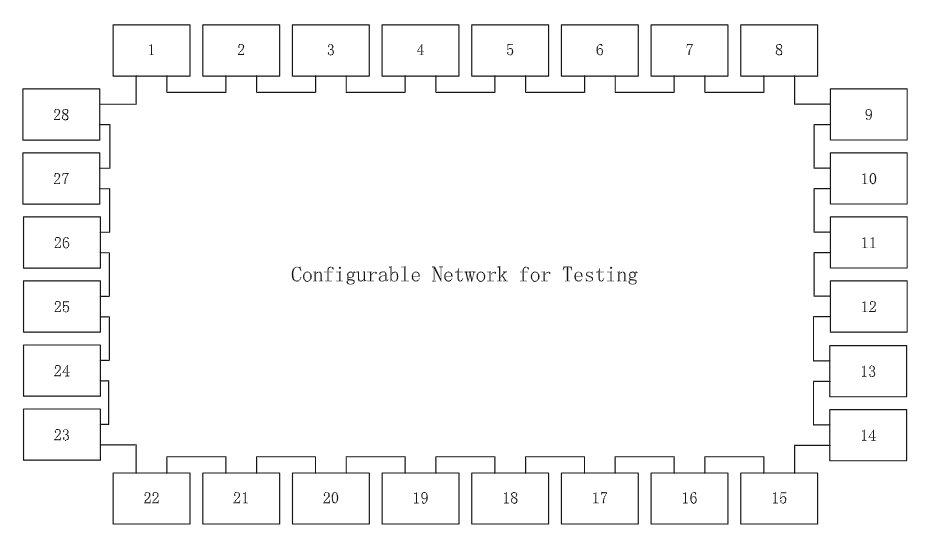
\includegraphics[scale=0.75]{Screenshot 2022-02-28 215019.png} 
\end{figure}
\begin{figure}[h]
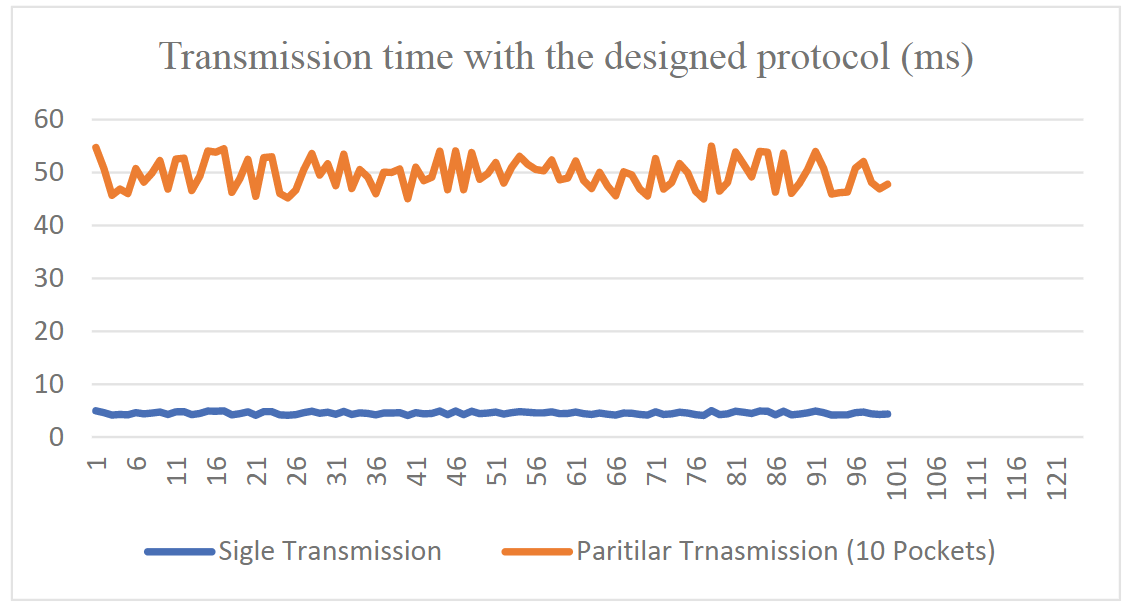
\includegraphics[scale=0.75]{Screenshot 2022-02-28 215029.png}
\end{figure}
\newpage
Service Time Analysis of Go-Back-N ARQ Protocol; FayzaA.Nada; Springer Nature Switzerland AG 2021; argues Automatic Repeat reQuest (ARQ) protocols are needed to control transmission errors at Data Link Layer (DLL) of OSI network model and to provide smooth and reliable transmission between network nodes. Using acknowledgements andtimeouts are essential in different types of ARQ protocols. Types of ARQ protocols include Stop-and-wait (SW) ARQ, Go-Back-N (GBN) ARQ,and Selective Repeat (SR) ARQ. The paper discusses Go-Back-N ARQ and Selective Repeat ARQ protocols and measures the service time of GBN ARQ protocol over unreliable channels. The distribution of service time has been analyzed as a stochastic process and the PGF of service time is obtained in terms of message size and error rate parameters. Moreover, first and second moments of service time distribution are presented. Results of the study can be implemented in studying and simulation of similar network models or approximation of relevant systems.
\\ \\
Data Link Layer Encryption for The Internet of Things Using Elliptic Curve Cryptography Over Visible Light Communication Channel; D. Ene, V.I.E. Anireh, D. Matthias; International Journal of Computer Sciences and Engineering, 2020; argues that The  Internet  as a fast-growing communication  infrastructure  comes  with additional  challenges of cybersecurity.  A few  techniques  have  been  created  to  provide  security  in  the  application,  transport,  or  network  layer  of  a  network.  Many organizations  have  worked  to provide  security  at  higher  OSI  layers, from application layer right down to the network layers, without  any  at  the  Data  Link  layer.  This  has  opened  up  many  systems  to  a  variety  of  compromises  and  attacks. In  this  study,  visible  light  communication  technology  for  fast  data  communication  and  secure  data transmission on the  data  link  layer using public-key cryptosystem are  discussed. The  visible  light communication technology consists  of  Light  Emitting  Diodes  (LED)  that  flicker  at  an  incredibly  high  frequency,  thereby  enabling  a  very  high-speed wireless  communication  and  an  elliptic  curve encryption component that carries  out an  integrated  encryption  scheme  using Elliptic Curve Integrated Encryption Scheme (ECIES) and a digital signature algorithm using Elliptic Curve Digital Signature Algorithm (ECDSA). For the data link layer security, the encryption procedure is applied to the communications server and the programmable circuit boards (PCB) controlling the visible light communication devices. While the complete system model was implemented  in  a  program,  a  prototype  of  the  architecture  was  implemented  on  a microFourQ-MSP-IAR  Embedded Workbench IDE-MSP430 7.12.4, and Wolfram Mathematica. Two advantages of visible light communication and public-key encryption were demonstrated: 1) providing security for the data link layer messages. 2) using VLC to speed up the encryption and decryption process in the data link layer

\end{document}
